

\vspace{-15pt}
\section{Ablation studies} \label{sec:ablation}

We perform several ablation studies to explore and validate our design choices for computing \gcam{} visualizations. 
This includes visualizing different layers in the network, understanding importance of ReLU in \eqref{eq:gcam}, analyzing different types of gradients (for ReLU backward pass), and different gradient pooling strategies.




\vspace{-8pt}
\subsection*{1. \gcam{} for different layers}

We show \gcam{} visualizations for the ``tiger-cat'' class at different convolutional
layers in AlexNet and VGG-16.
As expected, the results from \reffig{fig:conv_layers} show that localization
becomes progressively worse as we move to earlier convolutional layers.
This is because later convolutional layers better capture high-level semantic information
while retaining spatial information than earlier layers, that have smaller
receptive fields and only focus on local features.

\begin{figure*}[t!]
	\centering
    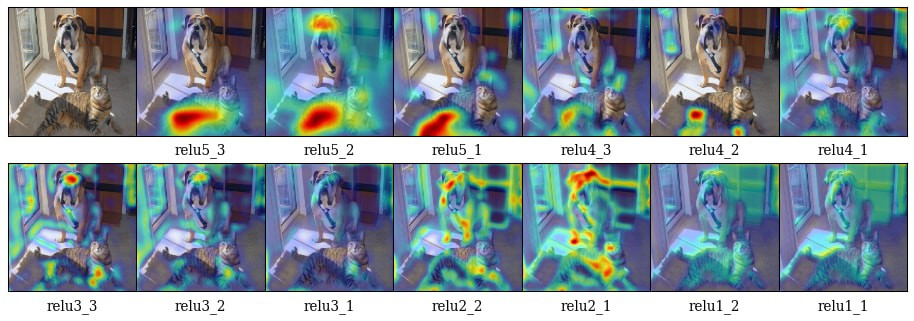
\includegraphics[width=1\textwidth]{figures/vgg16_conv_layers_new.jpg}\\
    \vspace{-5pt}
	 %
		\label{fig:vgg16conv}
        \vspace{5pt}
		\caption{ \gcam{} at different convolutional layers for the `tiger cat' class.
            This figure analyzes how localizations change qualitatively as we perform \gcam{} with respect to different feature maps in a CNN (VGG16~\cite{simonyan_arxiv14}).
	We find that the best looking visualizations are often obtained after the deepest convolutional layer in the network, and localizations get progressively worse at shallower layers.
This is consistent with our intuition described in Section 3 of main paper, that deeper convolutional layer capture more semantic concepts. %
}
	\label{fig:conv_layers}
\end{figure*}

\begin{figure*}
 \centering
 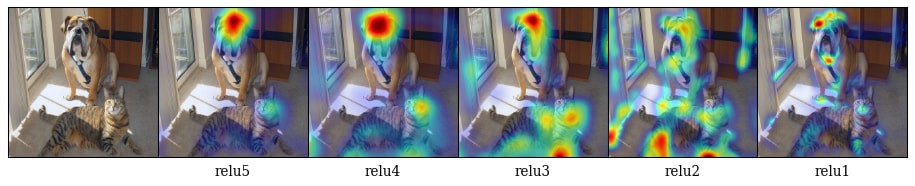
\includegraphics[width=1\linewidth]{figures/alex_conv_layers_new.jpg}
 \caption{\gcam{} localizations for ``tiger cat'' category for different rectified convolutional layer feature maps for AlexNet.}
 \label{fig:alex_conv}
\end{figure*}

\vspace{-5pt}
\subsection*{2. Design choices}

\vspace{-5pt}
\begin{table}[h!]
\centering
\captionsetup{belowskip=0pt,aboveskip=4pt}
    {
        \begin{tabular}{c@{\hskip 0.6in} c}\toprule
            \textbf{Method} & \textbf{Top-1 Loc error} \\
            \midrule

            \gcam{}                                                  & 59.65          \\
            \midrule
            \gcam{} without ReLU in Eq.1                             & 74.98          \\
            \gcam{} with Absolute gradients                          & 58.19          \\
            \gcam{} with GMP gradients                               & 59.96          \\
            \gcam{} with Deconv ReLU                                 & 83.95          \\
            \gcam{} with Guided ReLU                                 & 59.14          \\
            \bottomrule
        \end{tabular}

    }


    \caption{Localization results on ILSVRC-15 val for the ablations. Note that
    this evaluation is over 10 crops, while visualizations are single crop.}

    \label{table:locresablation}
\end{table}

We evaluate different design choices via top-1 localization errors on the ILSVRC-15
val set~\cite{imagenet_cvpr09}. See \reftab{table:locresablation}.
\subsubsection*{2.1. Importance of ReLU in \eqref{eq:scores}}

Removing ReLU (\eqref{eq:scores}) increases error by 15.3\%.
Negative values in \gcam{} indicate confusion between multiple occurring classes.






\subsubsection*{2.2. Global Average Pooling \vs Global Max Pooling}

Instead of Global Average Pooling (GAP) the incoming gradients to the convolutional layer,
we tried Global Max Pooling (GMP). We observe that using GMP lowers the localization ability
of \gcam{}. An example can be found in \reffig{fig:gmp} below. This may be due to the fact
that max is statistically less robust to noise compared to the averaged gradient.

\begin{figure}[h]

     \centering
     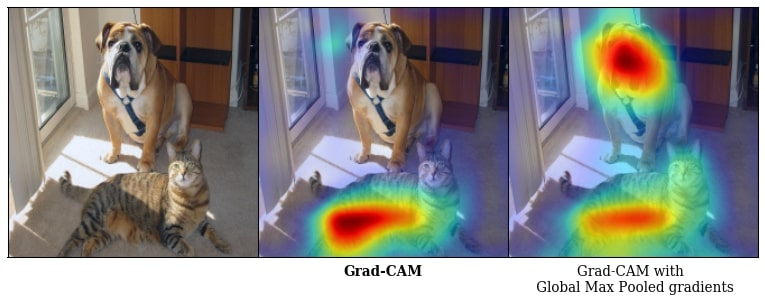
\includegraphics[width=1\linewidth]{figures/gcam_ablation_gap_gmp.jpg}
     \caption{\gcam{} visualizations for ``tiger cat'' category with Global Average Pooling and Global Max Pooling.}
     \label{fig:gmp}

   \end{figure}

\subsubsection*{2.3. Effect of different ReLU on \gcam{}}

We experiment with Guided-ReLU~\cite{springenberg_arxiv14} and Deconv-ReLU~\cite{zeiler_eccv14}
as modifications to the backward pass of ReLU.

\textbf{Guided-ReLU:} Springenberg~\etal\cite{springenberg_arxiv14} introduced Guided Backprop,
where the backward pass of ReLU is modified to only pass positive gradients
to regions of positive activations.
Applying this change to the computation of \gcam{} introduces a drop in the
class-discriminative ability as can be seen in \figref{fig:relu},
but it marginally improves localization performance as can be seen in \reftab{table:locresablation}.

\textbf{Deconv-ReLU:} In \dec{}~\cite{zeiler_eccv14}, Zeiler and Fergus introduced a
modification to the backward pass of ReLU to only pass positive gradients.
Applying this modification to the computation of \gcam{} leads to worse results
(\figref{fig:relu}). This indicates that negative gradients also carry
important information for class-discriminativeness.



\begin{figure}[h]

     \centering
     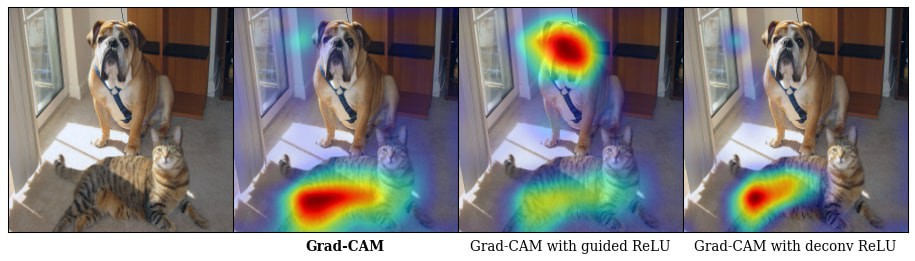
\includegraphics[width=1\linewidth]{figures/gcam_ablation_guided_deconv_ReLU.jpg}
     \caption{\gcam{} visualizations for ``tiger cat'' category for different modifications to the ReLU backward pass. The best results are obtained when we use the actual gradients during the computation of \gcam{}.}
     \label{fig:relu}
   \end{figure}


